\documentclass[12pt,a4paper]{ctexart}

\usepackage[UTF8]{ctex}
\usepackage{geometry}
\usepackage{graphicx}
\usepackage{xcolor}
\usepackage{tikz}
\usepackage{fontspec}
\usepackage{setspace}
\usepackage{enumitem}
\usepackage{booktabs}
\usepackage{array}
\usepackage{longtable}
\usepackage{hyperref}
\usepackage{fancyhdr}
\usepackage{titlesec}
\usepackage{multicol}
\usepackage{xurl}
\usepackage{tocloft}

\renewcommand{\cfttoctitlefont}{\hfill\bfseries\Large}
\renewcommand{\cftaftertoctitle}{\hfill}
\geometry{left=2.5cm,right=2.5cm,top=2.5cm,bottom=2.5cm}

\definecolor{black}{RGB}{0,0,0}
\definecolor{mainblue}{RGB}{0,82,147}
\definecolor{accentgold}{RGB}{180,140,60}
\definecolor{lightgray}{RGB}{245,245,245}
\definecolor{darkgray}{RGB}{80,80,80}
\definecolor{mainred}{RGB}{230,1,45}

\hypersetup{
    colorlinks=true,
    linkcolor=black,
    urlcolor=mainblue,
    citecolor=mainblue,
    pdfborder={0 0 0}
}

\pagestyle{fancy}
\fancyhf{}
\fancyhead[L]{\small\color{darkgray}\textbf{量子行业每周新闻洞察}}
\fancyhead[R]{\small\color{darkgray}\textbf{总第184期}}
\fancyfoot[C]{\thepage}
\renewcommand{\headrulewidth}{0.4pt}
\renewcommand{\footrulewidth}{0pt}

\titleformat{\section}
    {\Large\bfseries\color{mainred}}
    {\thesection、}{0em}{}
\titleformat{\subsection}
    {\large\bfseries\color{mainred}}
    {\thesubsection、}{0em}{}

\newcolumntype{L}[1]{>{\raggedright\arraybackslash}p{#1}}
\newcolumntype{C}[1]{>{\centering\arraybackslash}p{#1}}

\begin{document}

% ==================== 封面 ====================
\begin{titlepage}
\begin{tikzpicture}[remember picture,overlay]
    \fill[mainred] ([yshift=-0.5cm]current page.north west) rectangle ([yshift=-1.2cm]current page.north east);
    \fill[mainred] ([yshift=1.2cm]current page.south west) rectangle ([yshift=0.5cm]current page.south east);
\end{tikzpicture}

\vspace*{4cm}

\begin{center}
    {\fontsize{44}{52}\selectfont\bfseries\color{black} \textbf{量子行业每周新闻洞察}}

    \vspace{0.8cm}

    {\fontsize{16}{22}\selectfont\color{darkgray} 2026.06.14 — 2026.06.18 }
    {\fontsize{16}{22}\selectfont\color{darkgray} \textbf{WEEKLY NEWS}}

    \vspace{1.5cm}

    {\fontsize{20}{26}\selectfont\color{mainred}\textbf{（总第\textbf{ 184 }期）}}

    \vspace{4cm}

    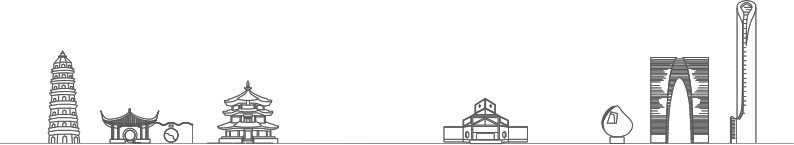
\includegraphics[width=\textwidth]{Cover_Suzhou.png}

    \vfill

    {\fontsize{12}{16}\selectfont\color{darkgray} 量子科技长三角产业创新中心\\编制：战略情报与成果专利室、产业发展部（理事会办公室）}
\end{center}
\end{titlepage}

% ==================== 目录 ====================
\pagenumbering{roman}
\newpage
\tableofcontents

\newpage

% ==================== 摘要 ====================
\pagenumbering{arabic}
\setcounter{page}{1}
\begin{center}
{\Large\bfseries\color{mainred} 摘\hspace{2em}要}
\end{center}
\addcontentsline{toc}{section}{摘要}


\textbf{ 宏观态势：}

全球量子技术竞争进入体系化布局阶段，各国加速构建本土生态与基础设施。美国智库评估中美差距正在缩小，促使西方阵营加大投入，德国、荷兰、以色列等国纷纷启动集成光子学、量子通信网络等关键研发项目。同时，国际合作呈现多极化趋势，金砖国家间、印俄间以及欧洲内部的量子教育联盟与数据中心框架相继建立，多所大学增设量子专业，标志着全球量子人才与产业链的储备竞赛全面升温。


\textbf{ 科技前沿：}

技术突破集中在量子纠错、极端材料探索与跨学科融合三大方向。微软与Quantinuum合作显著提升逻辑电路保真度，被动纠错等新方案有效延长了量子比特寿命，纠错技术正从理论走向可行。Kagome自旋冰、马约拉纳模式、准一维量子材料以及广义相对论与量子力学的桌面融合实验，展现了基础物理的新发现。此外，量子模拟已触及真实分子化学动力学，量子神经网络在临床数据、量子存储器在信息检索上均展现出超越经典的潜力，实用化进程加速。


\textbf{ 产品动态：}

量子计算硬件与核心材料正从实验室迈向工程化落地。容错量子计算机及氦量子系统平台等专用设备的发布与预订，标志着行业开始面向逻辑量子比特进行架构设计。高纯度硅-28的量产解决了芯片关键材料的自主难题，IBM开源费米子量子电路模拟库等软件工具降低了开发门槛。意大利及欧洲多地接连启用中性原子与超导量子计算机，后量子密码标准草案的推进，显示出计算平台与安全防护产品正同步走向成熟与商用。


\textbf{ 企业资讯：}

产业协同与场景渗透成为本周企业布局的主旋律。安全领域，Indra、EigenQ及ELECTRA AI分别针对防务、公共部门和电池智能系统展开后量子安全合作；计算应用端，Atom Computing与Phasecraft联合探索能源领域，IQM量子计算机投入超算中心运行。产业链方面，QuiX向量子计算公司交付首台通用光子计算机，日本团队在金刚石NV色心工艺上取得进展，显示出企业正通过垂直整合与跨界协作加速量子技术的商业化落地。


\textbf{ 资本运作：}

资本持续向量子计算产业化深水区注入动力，呈现“硬核早期”与“规模上市”并行的态势。国内太微量子、太一量生相继完成大额早期融资，北京首只量子产业子基金成立，政策与市场资本正合力扶持本土供应链。国仪量子即将登陆科创板，标志着量子精密测量赛道走向成熟。国际方面，风险投资聚焦超导芯片良率提升，多国政府精准资助量子密码、控制通信及算法研究，以资本牵引关键技术转化与商业护城河的构建。




\textbf{ 专利动态：}

本周专利动态涵盖低温环境系统、超导量子测控技术、量子软件与算法、量子算力网共4个板块、15条专利。




% ==================== 会议列表 ====================
{
    \newpage
    \section*{ 6月量子科技行业国内、国际会议}
    \addcontentsline{toc}{section}{ 6月量子科技行业国内、国际会议}
    \scriptsize
    \begin{longtable}{C{0.8cm}L{2.5cm}L{3cm}L{7cm}}
        \toprule[1.5pt]
        \textbf{序号} & \textbf{日期} & \textbf{地点} & \textbf{会议名称} \\
        \midrule
        \endfirsthead
        \toprule
        \textbf{序号} & \textbf{日期} & \textbf{地点} & \textbf{会议名称} \\
        \midrule
        \endhead
        \bottomrule
        \endfoot
        
        1 & 6月1日-3日 & 拉勒米, 美国 & 第四届怀俄明大学量子暑期学校 \\
        \midrule[0.05pt]
        
        2 & 6月1日-5日 & 罗利, 美国 & 2026量子机器学习暑期研讨会 \\
        \midrule[0.05pt]
        
        3 & 6月1日-5日 & 普罗维登斯, 美国 & 第57届APS原子、分子与光物理年会 \\
        \midrule[0.05pt]
        
        4 & 6月2日-4日 & 特隆赫姆, 挪威 & 量子自旋电子学 \\
        \midrule[0.05pt]
        
        5 & 6月3日-4日 & 罗切斯特, 美国 & 量子热力学与退相干 \\
        \midrule[0.05pt]
        
        6 & 6月4日-5日 & 东京, 日本 & Q2B：量子价值路线图 \\
        \midrule[0.05pt]
        
        7 & 6月5日 & 格拉斯哥, 英国 & 量子与社会研究研讨沙盒 \\
        \midrule[0.05pt]
        
        8 & 6月7日-12日 & 圣巴巴拉, 美国 & 第八届国际量子纠错会议 \\
        \midrule[0.05pt]
        
        9 & 6月7日-13日 & 克里特岛, 希腊 & 青年原子光学会议 \\
        \midrule[0.05pt]
        
        10 & 6月8日-11日 & 滑铁卢, 加拿大 & 量子光子学 \\
        \midrule[0.05pt]
        
        11 & 6月8日-20日 & 卡尔热斯, 法国 & 量子技术计算与通信暑期学校 \\
        \midrule[0.05pt]
        
        12 & 6月8日-8月14日 & 洛斯阿拉莫斯, 美国 & 2026洛斯阿拉莫斯量子计算暑期学校 \\
        \midrule[0.05pt]
        
        13 & 6月9日 & 巴黎, 法国 & Q-Day量子风险峰会：后量子密码学与量子密钥分发 \\
        \midrule[0.05pt]
        
        14 & 6月10日-12日 & 华沙, 波兰 & Perspektywy科技女性峰会 \\
        \midrule[0.05pt]
        
        15 & 6月10日-12日 & 多恩比恩, 奥地利 & 第四届砷化镓量子点国际研讨会 \\
        \midrule[0.05pt]
        
        16 & 6月10日-12日 & 埃朗根, 德国 & 神经形态计算前沿 \\
        \midrule[0.05pt]
        
        17 & 6月11日 & 杰克逊维尔, 美国 & 量子当下，医疗未来 \\
        \midrule[0.05pt]
        
        18 & 6月15日-17日 & 苏黎世, 瑞士 & 欧洲集成光学会议（ECIO） \\
        \midrule[0.05pt]
        
        19 & 6月15日-18日 & 格拉斯哥, 英国 & Optica Quantum 2.0会议 \\
        \midrule[0.05pt]
        
        20 & 6月15日-18日 & 赫尔辛基, 芬兰 & 仲夏开放量子系统、退相干及量子-经典交叉会议 \\
        \midrule[0.05pt]
        
        21 & 6月15日-18日 & 洛杉矶, 美国 & 量子器件设计研讨会 \\
        \midrule[0.05pt]
        
        22 & 6月16日 & 巴黎, 法国 & 第5届France Quantum \\
        \midrule[0.05pt]
        
        23 & 6月16日-17日 & 伦敦, 英国 & 第5届年度量子商业化全球大会2026 \\
        \midrule[0.05pt]
        
        24 & 6月16日-17日 & 格拉斯哥, 英国 & Optica 2026量子产业峰会——第5届 \\
        \midrule[0.05pt]
        
        25 & 6月21日-25日 & 塞费尔德, 奥地利 & 第57届欧洲原子系统组年度会议（EGAS 57） \\
        \midrule[0.05pt]
        
        26 & 6月21日-26日 & 塞费尔德, 奥地利 & 第7届塞费尔德量子信息研讨会 \\
        \midrule[0.05pt]
        
        27 & 6月21日-7月4日 & 贝纳斯克, 西班牙 & 量子科学：实现 \\
        \midrule[0.05pt]
        
        28 & 6月22日-24日 & 奥斯陆, 挪威 & IQT北欧：变化世界中的量子技术 \\
        \midrule[0.05pt]
        
        29 & 6月26日 & 汉堡, 德国 & 第7届ISC HPC国际研讨会——监控、可观测性与运营数据分析 \\
        \midrule[0.05pt]
        
        30 & 6月26日 & 汉堡, 德国 & 第2届统一计算中心量子资源研讨会（QRUCH） \\
        \midrule[0.05pt]
        
        31 & 6月26日 & 汉堡, 德国 & 第5届量子及混合量子/经典计算方法研讨会 \\
        \midrule[0.05pt]
        
        32 & 6月26日 & 汉堡, 德国 & 科学与工业数字孪生研讨会——从数据科学家到数据中心 \\
        \midrule[0.05pt]
        
        33 & 6月22日-7月3日 & 雷苏什, 法国 & 2026光子与原子暑期学校：量子气体、光-物质相互作用、量子技术 \\
        \midrule[0.05pt]
        
        34 & 6月23日-24日 & 罗马(纽约州), 美国 & 量子国际年度研讨会（Q4I） \\
        \midrule[0.05pt]
        
        35 & 6月23日-26日 & 阿尔加维, 葡萄牙 & 第3届量子安全网络与系统研讨会（QSNS 2026） \\
        \midrule[0.05pt]
        
        36 & 6月25日-26日 & 波士顿, 美国 & Quantum.Tech World \\
        \midrule[0.05pt]
        
        37 & 6月29日-7月1日 & 汉堡, 德国 & 国际计算科学大会量子计算专题 \\
        \midrule[0.05pt]
        
        38 & 6月29日-7月3日 & 贝桑松, 法国 & 第14届欧洲频率与时间研讨会（EFTS） \\
        \midrule[0.05pt]
        
        39 & 6月29日-7月10日 & 阿斯巴雷拉斯, 西班牙 & La Ricotta暑期学校：干草堆中的量子 \\
        \midrule[0.05pt]
        
        40 & 6月30日-7月1日 & 柏林, 德国 & GITEX欧洲 \\
        \midrule[0.05pt]
        
    \end{longtable}
}




% ==================== 宏观态势 ====================
\newpage
\section{宏观态势}
\vspace{-0.5em}
\noindent\rule{\linewidth}{1.5pt}

\subsection{ SEALSQ公司宣布在量子空间轨道云开发方面取得进展 }

SEALSQ Corp宣布量子空间轨道云(QSOC)取得重大进展。该平台利用卫星提供后量子安全服务，整合后量子密码学、量子随机数生成和可信AI处理。首颗卫星计划2026年Q4搭载SpaceX发射，目标2033年前建成百颗卫星星座。SEALSQ与WISeKey利用自2023年21次SpaceX发射中验证的技术，包括安全半导体和加密钱包，将运营云服务层。

\noindent\textbf{报道链接：}\url{https://www.globenewswire.com/news-release/2026/06/12/3311109/0/en/sealsq-and-wisekey-update-progress-on-their-post-quantum-security-cloud-from-space-through-the-quantum-spatial-orbital-cloud-qsoc.html}

\subsection{ 以色列斥资1.5亿新谢克尔启动集成光子学研发基础设施招标 }

2026年06月17日消息，以色列创新局与以色列国防部下属国防研发局（DDR\&D/MAFAT）联合发起一项新的项目招标，旨在建立或提供集成光子学领域的先进研发基础设施。施。该计划总投资额高达1.5亿新谢克尔，旨在加速以色列下一代光子芯片的研发进程，同时扩大工业界与学术界获取先进研发基础设施的渠道。

\noindent\textbf{报道链接：}\url{https://innovationisrael.org.il/en/press\_release/integrated-photonics-rnd/}

\subsection{ 美国智库：量子技术领域美国整体仍领先中国，但中国正系统性缩小差距 }

2026年06月17日消息，美国智库“特别竞争研究项目”（SCSP）发布的一份报告指出，美国目前在量子技术领域整体上仍略微领先于中国，但中国通过协调一致的国家战略正稳步缩小差距。距。该报告认为，美国在量子软件、纠错、私人投资及部分供应链环节保持优势，而中国在量子网络部署方面已处于领先地位，并在材料、制造和人才培养领域加速追赶。

\noindent\textbf{报道链接：}\url{https://thequantuminsider.com/2026/06/15/report-u-s-still-leads-in-quantum-technology-but-china-is-closing-the-gap/}

\subsection{ 德国启动CHIRON项目以构建基于纠缠的量子通信网络 }

2026年06月17日消息，一个名为CHIRON的量子通信基础设施项目在德国正式启动。启动。该项目由德国领先研究机构及技术企业联合推进，旨在构建一个可扩展的、基于纠缠的量子通信网络，以保护欧洲数字网络免受新兴网络威胁。项目得到了德国联邦教育与研究部（BMBF）资助，计划在柏林城区和图林根农村的两个真实测试平台上演示该网络，并将该量子通信基础设施集成至现有信息通信技术基础设施内。项目还将在德国联邦政府机构内测试量子安全访问令牌，以扩展至公共管理、关键基础设施及金融服务等领域。

\noindent\textbf{报道链接：}\url{https://thequantuminsider.com/2026/06/15/chiron-project-launches-quantum-communication-network-initiative/}

\subsection{ 荷兰NWO将启动量子安全项目征集，聚焦量子纠缠网络与后量子密码双路线 }

2026年06月17日消息，荷兰研究理事会（NWO）将于7月启动“量子时代的安全与韧性”项目征集，邀请研究人员在量子网络纠缠与后量子密码学领域开展基础研究。据了解，此次征集分为两条研究路线：路线一聚焦量子网络中“可便携”纠缠的应用，目标是探索在单点生成纠缠后长期存储于便携式量子存储器中的解决方案；路线二聚焦后量子密码学，旨在增进对现有及新型抗量子密码技术的认知与信心。

\noindent\textbf{报道链接：}\url{https://www.nwo.nl/en/news/pre-announcement-call-on-future-proof-quantum-technology}

\subsection{ 首届金砖国家量子技术论坛于日前在莫斯科召开，俄白两国将深化量子技术领域的合作 }

2026年06月15日消息，首届金砖国家量子技术论坛在莫斯科举行，来自科学界、产业界和政府部门的专家齐聚一堂，共同探讨量子技术领域的合作前景。景。该论坛指出，量子技术是当今未来技术发展的重中之重，主要可合作的方向包括科学研究、量子计算应用、人才培养、量子专业劳动市场建设，以及量子技术在核能领域的应用。白俄罗斯官员在会上表示，该国已与俄罗斯在量子技术领域已有丰富的合作经验，双方计划在此基础上进一步拓展合作。

\noindent\textbf{报道链接：}\url{https://belarus24.by/en/news/economy/belarus-and-russia-to-develop-projects-in-the-field-of-quantum-technologies/}

\subsection{ 韩国浦项科技大学正式成立量子全球合作伙伴引领中心 }

2026年06月16日消息，韩国科学技术信息通信部宣布，在浦项科技大学（POSTECH）正式成立“量子全球合作伙伴引领中心”。”。该中心旨在开发跨多种量子计算平台的大规模量子纠缠技术，它将作为韩国与海外研究机构合作的枢纽，合作方包括哈佛大学和麻省理工学院。这一举措标志着韩国在推动量子技术国际化合作方面迈出重要一步，有望加速量子计算领域的关键突破。

\noindent\textbf{报道链接：}\url{https://www.telecompaper.com/news/south-korea-launches-quantum-research-centre-with-harvard-mit-partnerships--1573487}

\subsection{ 印度寻求与俄罗斯进行量子计算合作，以实现2030年国家量子任务目标 }

2026年06月16日消息，印度驻俄罗斯大使Vinay Kumar在莫斯科举行的金砖国家量子技术论坛上表示，印度正寻求与俄罗斯在量子计算领域展开合作，以实现其国家量子任务（NQM）在2030—2031年间的目标。标。NQM任务预算为7.3亿美元，旨在构建完整的国家量子生态系统，涵盖中等规模量子计算机、量子通信网络以及量子材料与组件等关键领域。

\noindent\textbf{报道链接：}\url{https://russiaspivottoasia.com/india-proposes-quantum-computing-collaboration-with-russia/}

\subsection{ 巴塞罗那大学新量子实验室启用，将助力高水平科研与教学工作 }

2026年06月16日消息，巴塞罗那大学物理学院启用了一个专注于量子科学教学与研究的学术实验室，以支持高水平的实验工作。作。该设施将推动该校量子学科领域的发展，巴塞罗那大学还参与了新启动的欧洲量子学院（EQA）项目，也将为这一领域注入了更强动力。该实验室设备得到了加泰罗尼亚量子学院的支持，后者是加泰罗尼亚政府推动的“Quàntica：地中海科学与量子技术谷”计划的一部分。

\noindent\textbf{报道链接：}\url{https://web.ub.edu/en/web/actualitat/w/laboratory-quantum-sciences?tn=np\&referer=press-releases}

\subsection{ BW Digital将与新加坡国立大学合作构建适用于东南亚的量子就绪数据中心框架 }

2026年06月16日消息，BW Digital与新加坡国立大学设计与工程学院近日启动了一项研究合作，致力于为东南亚地区开发量子就绪的数据中心基础设施框架。这项为期18个月的项目将研究量子-经典计算集成所需的物理基础设施条件，包括热管理、低温系统、电力供应、网络连接及运维等关键考量。团队将重点分析热带环境对量子基础设施部署的影响，并据此开发规划工具及面向未来设施的量子就绪框架。

\noindent\textbf{报道链接：}\url{https://thequantuminsider.com/2026/06/11/bw-digital-and-nus-to-advance-quantum-ready-data-centres-for-southeast-asia/}

\subsection{ 欧洲量子学院正式启航，ICFO将携手共筑欧洲量子教育新生态 }

欧洲量子学院(EQA)正式启动，ICFO将协调西班牙和葡萄牙10个机构的西南欧区域量子学院。EQA通过六个区域学院覆盖全欧，旨在弥合“量子鸿沟”，协调从学校到终身学习的教育链。项目目标培训至少600名量子专业人员、5000名学习者，并将20\%差旅补助分配给代表性不足群体。

\noindent\textbf{报道链接：}\url{https://www.icfo.eu/news/2674/a-new-quantum-academy-to-forge-the-workforce-of-tomorrow/880/}

\subsection{ 澳大利亚量子计算未来领导者培训中心在悉尼大学正式启动 }

澳大利亚研究理事会量子计算未来领导者培训中心(FLiQC)在悉尼大学启动，获5年500万澳元资助。中心主任为斯蒂芬·巴特利特教授。FLiQC聚焦量子器件、架构和算法，培养量子计算人才，连接研究与国防、物流等行业应用。

\noindent\textbf{报道链接：}\url{https://www.arc.gov.au/news-and-publications/media/australia-invests-future-quantum-computing-leaders}

\subsection{ 印度Wadhwani-IISc创新中心成立，量子初创企业加速平台InQubate同时启动 }

印度科学研究所(IISc)瓦德瓦尼创新中心落成，作为瓦德瓦尼创新网络(投资超140亿卢比)一部分。同时举办2026年量子推介会并启动InQubate量子初创企业加速平台，由四元生态系统支持，旨在推动深度科技转化。

\noindent\textbf{报道链接：}\url{https://www.iisc.ac.in/events/strengthening-indias-quantum-and-deep-tech-innovation-ecosystem-with-launch-of-wadhwani-iisc-innovation-centre/}

\subsection{ 印度理工学院曼迪分校宣布下学年将新增量子科学与工程等三大本科专业 }

2026年06月15日消息，印度理工学院曼迪分校（IIT Mandi）近日宣布，该校自下个学年起将新增三个本科专业：量子科学与工程、农业工程（数据分析方向）、化学工程（数据分析方向）。其中，量子科学与工程专业课程涵盖量子计算、量子通信、传感技术、先进材料、硬件工程、计算机科学、数学及人工智能等核心领域。这一举措旨在培养跨学科人才，满足量子科技及数据驱动工程领域日益增长的需求。

\noindent\textbf{报道链接：}\url{https://www.hindustantimes.com/education/news/iit-mandi-launches-b-tech-programme-in-quantum-science-and-engineering-101780914168301-amp.html}


% ==================== 科技前沿 ====================
\newpage
\section{科技前沿}
\vspace{-0.5em}
\noindent\rule{\linewidth}{1.5pt}

\subsection{ 微软与Quantinuum合作取得新突破：逻辑电路错误率降低800倍 }

微软在《自然》发文，展示在Quantinuum离子阱硬件上实现逻辑错误率比物理基线降低11-800倍。团队展示了12个逻辑量子比特的容错计算。微软量子平台支持离子阱、中性原子和拓扑量子比特，并推出开源纠错软件包“deq”。

\noindent\textbf{报道链接：}\url{https://quantum.microsoft.com/en-us/insights/blogs/microsoft-application-of-error-correction-to-trapped-ion-qubits}

\subsection{ 在Kagome自旋冰中实现的非线性磁响应 }

奥格斯堡大学物理学家在HoAgGe材料中发现非线性磁化率可探测时间反演对称性破缺，实现对简并自旋冰畴操控。研究利用极化中子散射确定其三维XY普适性相变，为受挫磁体基础研究及信息技术应用带来新见解。

\noindent\textbf{报道链接：}\url{https://www.uni-augsburg.de/en/campusleben/neuigkeiten/2026/06/12/non-linear-magnetic-response-realized-in-kagome-spin-ice/}

\subsection{ 布鲁克海文国家实验室科学家利用超快激光脉冲揭示材料隐藏的物质状态 }

布鲁克海文国家实验室科学家利用飞秒激光脉冲，将锰氧化物从绝缘态切换至一种隐藏的导电态。因其非热力学路径达至，被称为“隐藏”相，且状态持续。该研究利用RIXS和XAS技术，为未来量子器件设计控制了新方向。

\noindent\textbf{报道链接：}\url{https://www.bnl.gov/newsroom/news.php?a=222971}

\subsection{ 印度量子网络安全公司QNu Labs与埃因霍温理工大学签署研究协议 }

2026年06月17日消息，近日，印度量子初创公司QNu Labs与荷兰埃因霍温理工大学正式达成一项研究合作，将在ACE QKD项目下测试、验证并增强量子密钥分发系统在规模化部署中的长期韧性。此外，QNu Labs还宣布与SAGA Consultants签署战略协议，旨在通过国际合作来推动量子安全技术在银行与金融服务领域的应用拓展。

\noindent\textbf{报道链接：}\url{https://thequantuminsider.com/2026/06/15/qnu-labs-takes-indias-quantum-cybersecurity-to-bharat-innovates-2026-signs-research-deal-with-eindhoven-university-of-technology/}

\subsection{ 马萨诸塞大学研究人员开发的被动纠错技术能让量子比特寿命翻倍 }

2026年06月17日消息，美国马萨诸塞大学阿默斯特分校的研究人员设计出一种被动量子纠错技术，可使量子比特能够自行纠正错误。该方案将量子比特系统中不可避免的能量耗散从障碍转化为优势，为实验室外的实用量子计算开辟了可行路径。实验结果显示，该协议能将量子比特的寿命延长至196微秒，是未应用被动纠错量子比特寿命的2.15倍，且这一数值几乎正好达到此前被动方案从未实现的盈亏平衡点。该方法有望为实现实用且有韧性的量子比特提供一条有前景的路径。相关成果已于日前发表在《物理评论X》上。

\noindent\textbf{报道链接：}\url{https://phys.org/news/2026-06-passive-quantum-error-qubit-lifetime.html}

\subsection{ 美国加州大学的研究团队在准一维量子材料领域取得新成果 }

2026年06月17日消息，美国加州大学洛杉矶分校与河滨分校的研究人员展示了一种新型准一维量子材料的潜力，该材料可显著增强对电荷密度波（CDW）这类集体电子态的电控能力。该研究阐述了一种强大的机制，能够可靠地控制集体电子态，有望为开发新型低功耗电子器件提供重要支持。他们的这一成果为量子材料在实际电子系统中的应用开辟了新路径。相关研究论文已于日前发表在《自然电子学》上。

\noindent\textbf{报道链接：}\url{https://phys.org/news/2026-06-quasi-1d-material-electric-standard.html}

\subsection{ 欧洲首台在同步辐射源运行的TES光谱仪上线，光子探测效率提升超百倍 }

2026年06月17日消息，近日，欧洲唯一一台在同步辐射源上运行的TES光谱仪已在德国BESSY II同步辐射装置中运行。该仪器由德国亥姆霍兹柏林材料与能源中心、马克斯·普朗克化学能转换研究所以及美国国家标准与技术研究院合作开发。这台基于超导过渡边缘传感器（TES）阵列的光子探测器，通过稀释制冷机实现了低于25毫开尔文的工作温度，在光子探测效率上比传统波长色散型X射线发射光谱仪要高出100至1000倍。

\noindent\textbf{报道链接：}\url{https://www.helmholtz-berlin.de/pubbin/news\_seite?nid=34306\&seitenid=74699\&sprache=en}

\subsection{ 新实验与理论研究证实：马约拉纳模式对无序具有高度鲁棒性 }

2026年06月16日消息，德国汉堡大学的研究人员与合作者进行的一项新项研究专门探索了一维自旋链中编码的马约拉纳模式的鲁棒性。他们实验证明了这些原子链中的马约拉纳模式确实能抵抗无序干扰，进一步凸显了其在实现容错量子计算方面的潜力。研究人员表示，该研究最激动人心的成果是他们直接通过实验与理论双重证实，马约拉纳准粒子对多种类型和程度的无序具有高度鲁棒性。相关成果已于日前发表在《自然物理学》期刊。

\noindent\textbf{报道链接：}\url{https://phys.org/news/2026-06-majorana-modes-disorder-atomic-chains.html}

\subsection{ 微软与Quantinuum合作演示量子纠错技术可大幅降低计算错误率 }

2026年06月16日消息，微软量子部门与量子计算公司Quantinuum近日在《自然》杂志上发表了一项合作研究，证明了量子纠错技术能将计算错误率降低至使用物理量子比特直接计算的11分之一到800分之一。他们采用名为“碳码”和“tesseract码”的两种纠错方法，在涉及最多12个逻辑量子比特的实验中，成功实现了计算过程中的重复纠错，并获得了更低的逻辑错误率。研究人员表示，这一结果表明当前量子处理器已能受益于容错能力，但要实现实用化的大规模量子计算机，仍需在硬件、实时解码和可扩展的纠错方法上取得进一步突破。

\noindent\textbf{报道链接：}\url{https://thequantuminsider.com/2026/06/13/microsoft-and-quantinuum-report-on-major-gains-in-quantum-error-correction/}

\subsection{ 悉尼大学科学家首次对真实分子的化学动力学进行了量子模拟 }

2026年06月15日消息，悉尼大学的研究人员最近首次对真实分子的化学动力学进行了量子模拟，相关成果已于日前发表在《美国化学会志》上。该研究通过模拟分子受光激发后的行为，推动了该领域的前沿发展，这一过程涉及超快电子与振动变化，传统计算机难以准确或高效建模。此次实验成功将量子模拟从理论推向了真实复杂分子领域，有望为药物设计、光化学反应机理研究及材料科学提供全新的计算路径。

\noindent\textbf{报道链接：}\url{https://www.sydney.edu.au/news-opinion/news/2025/05/15/quantum-simulation-of-chemical-dynamics-achieved-for-the-first-t.html}

\subsection{ 瑞典团队成功在动态可重构电信网络中部署远距离量子密钥分发链路 }

2026年06月15日消息，由瑞典林雪平大学、瑞典皇家理工学院、斯德哥尔摩大学和查尔姆斯理工大学组成的研究团队，近日在arXiv上发布了一项预印本研究，报告了将远距离可信节点量子密钥分发（QKD）链路物理部署到动态可重构电信网络中的现场试验。该网络拓扑连接了林雪平大学的一个实验室与斯德哥尔摩的国家量子中心，通过一个中间可信节点，将标准长距离单模光纤与多芯光纤接入段相结合，以模拟异构企业基础设施。该试验总距离达303公里，覆盖瑞典东南部。实验中，团队采用了一套改装的ThinkQuantum商用QKD系统，为其加装了外部超导纳米线单光子探测器。

\noindent\textbf{报道链接：}\url{https://quantumcomputingreport.com/field-demonstration-of-trusted-node-qkd-over-deployed-single-mode-and-multi-core-fiber-infrastructure/}

\subsection{ 密歇根大学科学家在一个桌面实验中巧妙融合了广义相对论与量子力学 }

2026年06月15日消息，美国密歇根大学的一个研究团队展示了一项将广义相对论与量子力学两大基础物理理论相结合的桌面实验，为探索二者在微观与宏观尺度下的交汇点提供了新路径。研究团队利用紧凑型光纤线圈构建了一台高度稳定的、可桌面操作的50公里光学干涉仪，并以单光子进行了测试。该团队的独特设计成功探测到一个足够小、由引力诱导相位信号，并达到了在实验室规模下测量引力红移（广义相对论的预测之一）所需的精度。研究人员表示，研究引力在真正量子系统中的效应，有助于揭示这两大理论在该领域是否完全兼容，并有可能为发现新物理学指明方向。相关成果已发表于近期的《物理评论快报 》期刊。

\noindent\textbf{报道链接：}\url{https://phys.org/news/2026-06-tabletop-fundamental-physics.html}

\subsection{ Multiverse Computing在大规模量子多体模拟领域取得重大突破 }

2026年06月15日消息，Multiverse Computing的科学家近日在大规模量子多体模拟领域取得重大突破，证明了先进的张量网络方法能够触及此前被认为超出经典计算能力范围的领域。该团队在一项新研究中开发出高度优化的模拟框架，结合了U(1)×SU(2)对称性保持的张量网络、GPU加速和先进的时间相关变分原理（TDVP）算法，利用四块英伟达H200 GPU，他们实现了约62,000的键维数，是实时量子动力学TDVP模拟中报告的最大键维之一，从而使经典方法能够完全收敛地模拟此前未能解决的一维费米-哈伯德模型。

\noindent\textbf{报道链接：}\url{https://multiversecomputing.com/resources/pushing-the-classical-frontier-of-quantum-simulation}

\subsection{ 科学家开发出量子神经网络训练框架，并在离子阱系统上验证了临床数据表现 }

2026年06月15日消息，一组国际研究团队开发出一种量子神经网络训练框架，能够在量子硬件上直接进行基于梯度的优化，且在临床数据集上的表现与强经典补值方法相当。该框架结合了蝴蝶电路架构、逐层训练以及并行化梯度估计技术，能显著减少训练过程中所需的量子电路评估次数。在研究中，团队利用IonQ的Forte Enterprise离子阱系统，展示了16量子比特的机上训练以及32量子比特的混合量子-经典模型推理，并将其应用于临床数据插补与患者生存预测任务。这一成果降低了量子机器学习中梯度计算成本这一关键障碍。相关论文已于日前在预印本服务器arXiv上的发表。

\noindent\textbf{报道链接：}\url{https://thequantuminsider.com/2026/06/09/researchers-demonstrate-scalable-quantum-neural-network-training-on-quantum-hardware/}

\subsection{ 东京大学新研究表明：量子存储器在检索未知信道方面要显著优于经典存储器 }

2026年06月15日消息，日本东京大学的一个研究团队近日在《物理评论快报》上发表一项成果，证明量子方法在存储和检索未知等距信道方面要显著优于经典方法。该团队评估了量子存储器在执行一种非经典任务（即存储和检索未知等距信道）时的表现。研究表明，在达成相同目标所需使用未知操作的次数上，量子策略实现了相对于最佳经典策略的平方级提升。该研究成果提供了一个严格的理论示例，证明量子存储器在存储和检索未知量子操作方面要优于经典存储器。

\noindent\textbf{报道链接：}\url{https://phys.org/news/2026-06-quantum-memory-surpasses-classical-limits.html}

\subsection{ 我国科研人员开发出一种基于超导量子比特的高精度量子传感方法 }

2026年06月15日消息，北京量子信息科学研究院联合电子科技大学、中国科学院物理研究所等机构的研究人员，展示了一种基于超导量子比特的高精度量子传感方法。该方法将非平衡动力学与量子临界性结合在Stark-Wannier局域化系统中，利用9超导量子比特链中量子激发的传播模式，实现了对梯度场强度的量子极限精度测量。相关成果已于近日在《科学通报》上发表。

\noindent\textbf{报道链接：}\url{https://www.eurekalert.org/news-releases/1131413}

\subsection{ 威斯康星大学研究人员开发出可用于中红外光谱分析的新型动态可调超表面 }

威斯康星大学麦迪逊分校Filiz Yesilköy团队开发出动态可调超表面，用于中红外光谱分析。通过集成微型加热器，可调谐光学共振扫描不同分子指纹，无需样品直接接触，为便携式生化传感器小型化迈出关键一步。

\noindent\textbf{报道链接：}\url{https://engineering.wisc.edu/news/tunable-metasurface-could-bring-powerful-molecular-sensing-from-the-lab-to-the-field/}

\subsection{ 日本研究人员开发出可利用激光进行重写的新型磁性存储材料 }

日本QST领导团队开发出新型磁性材料CoFeB人造亚铁磁体，可通过单次飞秒激光脉冲进行全光开关，实现数据重写。速度快于传统方法约1000倍且功耗更低，在NanoTerasu同步辐射设施完成分析，有望用于AI硬件和光电平台。

\noindent\textbf{报道链接：}\url{https://www.eurekalert.org/news-releases/1131699}

\subsection{ 爱尔兰东南理工大学将参与Rinn量子信息科学与技术研究中心的工作 }

爱尔兰通过爱尔兰研究局投资4.6亿欧元，成立七个Rinn研究中心，覆盖AI、量子、半导体等战略领域。东南理工大学将参与其中三个中心。该网络预计支持超577个研究职位，涵盖17所机构，并撬动额外5亿欧元投资。

\noindent\textbf{报道链接：}\url{https://www.setu.ie/news/setu-researchers-to-play-key-role-in-new-460-million-national-research-investment}

\subsection{ 德国研究人员发现光会导致量子摩擦从而减缓纳米材料的运动速度 }

波鸿鲁尔大学团队发现光致量子摩擦现象。在水溶液中，光激发使碳纳米管运动减慢。研究表明，管内激子与水分子集体运动直接耦合产生动量传递，可通过光控制固液界面摩擦，成果发表于《自然》。

\noindent\textbf{报道链接：}\url{https://news.rub.de/english/press-releases/2026-06-11-physical-chemistry-light-brake}

\subsection{ JILA与布鲁克大学研究人员合作演示镱原子作为量子比特的多用途性 }

JILA及因斯布鲁克大学团队展示镱-171原子可作为“变色龙”量子比特。实验在光学、里德伯和核量子比特间移动量子态，实现模拟、计算与计量功能连接。团队成功生成并传输多达20个里德伯量子比特的GHZ态。

\noindent\textbf{报道链接：}\url{https://www.colorado.edu/jila/2026/06/11/chameleon-atoms-jila-researchers-demonstrate-versatile-atomic-qubits-can-pass-around}

\subsection{ 瑞典六所大学联合成立瑞典量子技术中心 }

瑞典六所大学(包括乌普萨拉、查尔姆斯)联合成立瑞典量子技术中心，作为国家级量子技术枢纽，旨在通过协调研究、教育和创新，提升瑞典国际竞争力，避免资源分散。

\noindent\textbf{报道链接：}\url{https://www.uu.se/en/news/2026/2026-06-11-new-centre-to-strengthen-sweden-in-the-quantum-race}


% ==================== 产品动态 ====================
\newpage
\section{产品动态}
\vspace{-0.5em}
\noindent\rule{\linewidth}{1.5pt}

\subsection{ QuEra推出首台容错量子计算机，计划于2028年部署到亚马逊Braket平台 }

2026年06月17日消息，QuEra Computing日前宣布推出其首台容错量子计算机Libra，计划于2028年部署在亚马逊AWS的Braket云平台上。同时，QuEra还宣布与AWS深化双方的多年技术和市场合作，旨在向全球客户提供容错量子计算能力。作为双方扩展合作后的首款产品，Libra属于Megaquop级系统，目标是可执行约一百万次可靠的逻辑量子操作。其技术指标预计将超过256个纠错逻辑量子比特，逻辑错误率低至10⁻6。2028年起，AWS客户将可通过云平台访问这一容错量子计算系统，以支持早期的商业实践与科研工作流。

\noindent\textbf{报道链接：}\url{http://quera.com/press-releases/quera-announces-2028-fault-tolerant-quantum-computer-and-expanded-multi-year-strategic-collaboration-with-aws}

\subsection{ 我国科学家成功量产高纯度硅-28，量子芯片核心材料实现自主突破 }

2026年06月17日消息，近日，中核集团旗下中国原子能工业有限公司的科学家在稳定同位素富集与高纯硅制备领域取得关键突破，成功实现了丰度超过99.99\%的硅-28同位素的自主量产，产品关键指标达到国际先进水平。据了解，硅-28作为硅的稳定同位素，因原子核自旋为零、可大幅降低量子计算中的环境噪声干扰，被誉为“世界上最纯的硅”，是硅基量子芯片不可或缺的核心材料。

\noindent\textbf{报道链接：}\url{https://news.qq.com/rain/a/20260615A04GWL00}

\subsection{ IBM发布可用于快速模拟费米子量子电路的开源Python库 }

2026年06月16日消息，近日，IBM正式发布了一款用于快速模拟费米子量子电路的开源Python库“ffsim”。该库通过利用物理对称性来降低模拟成本和内存需求，使其能够完成通用量子模拟器无法实现的模拟任务，并且与Qiskit进行了集成以支持端到端的量子计算工作流。在针对分子哈密顿量的Trotterized时间演化的基准测试中，ffsim相较于FQE库快了一个数量级，而Qiskit Aer在更大系统规模下明显落后于两者。

\noindent\textbf{报道链接：}\url{https://www.ibm.com/quantum/blog/ffsim}

\subsection{ NIST发布个人身份验证标准初步草案，以推动后量子密码学应用落地 }

2026年06月16日消息，美国国家标准与技术研究院（NIST）近日发布了对个人身份验证（PIV）标准的初步工作草案，以支持后量子密码学（PQC）的应用。这些草案明确了使用ML-DSA数字签名算法和ML-KEM密钥封装机制来配合PIV所需的变化。当前草案包括SP 800-73第1部分、第2部分及SP 800-78，并附带一份PQC概览文件。

\noindent\textbf{报道链接：}\url{https://www.nist.gov/news-events/news/2026/06/working-drafts-post-quantum-cryptography-updates-piv-standards}

\subsection{ Horizon Quantum宣布将都柏林作为其第二套量子计算机的部署地 }

Horizon Quantum宣布在爱尔兰都柏林部署其第二套量子计算机，为IonQ 256量子比特系统。计划扩大当地团队，深化与本地量子生态系统合作，强化其软件基础设施与离子阱系统集成。

\noindent\textbf{报道链接：}\url{https://www.horizonquantum.com/resources/newsroom/horizon-quantum-announces-dublin-as-its-second-quantum-computer-testbed-location-bringing-a-frontier-quantum-system-to-ireland}

\subsection{ Alice \& Bob推出氦量子系统平台，用于量子纠错与逻辑量子比特研究 }

Alice \& Bob发布氦量子系统，这是一个可本地部署的完整猫量子比特系统。18个猫量子比特即可编码首个逻辑量子比特，功耗约40千瓦，通过开源QRMI库集成经典资源，旨在减少纠错开销。

\noindent\textbf{报道链接：}\url{https://www.hpcwire.com/off-the-wire/alice-bob-introduces-helium-platform-for-quantum-error-correction-and-logical-qubit-research/}

\subsection{ Pasqal启用意大利首台中性原子量子计算机，系其在欧洲部署的第三套系统 }

Pasqal在意大利CINECA启用其140量子比特中性原子量子计算机SOL。系统命名源于罗马太阳神，与Leonardo超算集成，通过QRMI构建混合工作流。这是其欧洲第三台部署的EuroHPC系统，由欧盟和意大利共资。

\noindent\textbf{报道链接：}\url{https://www.pasqal.com/newsroom/pasqal-inaugurates-italys-first-neutral-atom-quantum-computer-third-pasqal-system-in-europe/}

\subsection{ 第6台EuroHPC量子计算机SOL在意大利启用，总采购成本为1300万欧元 }

EuroHPC JU在意大利启用两台新系统：Pasqal的140量子比特量子计算机SOL，以及Leonardo超算的AI优化分区LISA(含1328个GPU)。两者集成于CINECA，由意大利和欧盟共资，旨在加强欧洲HPC和量子技术主权。

\noindent\textbf{报道链接：}\url{https://www.eurohpc-ju.europa.eu/inauguration-sol-new-quantum-computer-together-lisa-upgrade-leonardo-supercomputer-2026-06-11\_en}



% ==================== 专利动态 ====================
\newpage
\section{专利动态}
\vspace{-0.5em}
\noindent\rule{\linewidth}{1.5pt}

\subsection{ 低温环境系统 }

\subsubsection{ 一种具有异常检测功能的低压配电柜用量子通信终端设备 }

申请人：无锡鼎全量子科技有限公司

发明人：张超然 | 张万生

公开日/授权日：2026-06-16

摘要：

本实用新型公开了一种具有异常检测功能的低压配电柜用量子通信终端设备，包括低压配电柜柜体，所述低压配电柜柜体的内部下方设置有支撑架，所述支撑架的顶端安装有量子安全交换机，所述量子安全交换机的两侧外壁上分别开设有用于对所述量子安全交换机内部进行通风散热的进风口和出风口，且进风口和出风口处均设置有用于对外部空气中的杂质进行过滤的过滤网，所述量子安全交换机的一侧外壁上设置有异常检测机构，所述量子安全交换机顶端的中心位置设置有声光报警器。本实用新型有效的避免了因量子安全交换机通风散热异常而导致量子安全交换机产生过热故障的情况发生，延长了量子安全交换机的使用寿命，降低设备维护成本与更换频率。

\noindent\textbf{专利链接：}\url{https://analytics.zhihuiya.com/patent-view/abst?patentId=3fdfa899-0497-44a4-bea3-080a2fe71104&shareId=E960GD7C-5881-73D3-C2B5-98CEG0D1D628&from=EXPORT&signature=urXIgWq39P0YoQ3%2BJ8zBDqOPIGK8CJebAOg%2Fp0ZDcRo%3D&expire=94608000&date=20260618T015652Z&version=1.0}

\subsubsection{ 一种基于LNG-ANG耦合条件下的BOG回收系统及方法 }

申请人：中国石油大学(华东)

发明人：陈树军 | 熊轩 | 付越 | 陈灵丽 | 付益铭 | 郑龙

公开日/授权日：2026-06-16

摘要：

本发明属于清洁能源储存与高效利用技术领域，具体涉及一种基于LNG‑ANG耦合条件下的BOG回收系统及方法。本发明通过LNG‑ANG深度耦合技术，构建了包含LNG变物性特征与吸附床层动边界特征的热质传递耦合模型，基于该模型的动态调控，实现了LNG冷媒从粗放冷却向“冷量按需供给”的精准控制的跨越，避免了冷量浪费或移热不足，显著降低了系统能耗。建立了完整的“监测‑反演‑调控”闭环控制策略，显著延长了吸附剂的循环使用寿命，本发明引入㶲效率，将能量品位匹配作为优化目标，实现了从“能量守恒”到“㶲平衡”的理论跨越，使系统运行在热力学最优工况，实现了能量的高效梯级利用。

\noindent\textbf{专利链接：}\url{https://analytics.zhihuiya.com/patent-view/abst?patentId=42d0158d-3030-4d08-b42c-eafefff34285&shareId=E960GD7C-5881-73D3-C2B5-98CEG0D1D628&from=EXPORT&signature=iqKjmmjm3fcImh%2FvbFPCZz8aYb08u%2FcyOJVPkGYAHKo%3D&expire=94608000&date=20260618T015652Z&version=1.0}


\subsection{ 超导量子测控技术 }

\subsubsection{ 一种基于3×3对称约束矩阵的高维量子编码与容错纠错方法及系统 }

申请人：付志伟

发明人：付志伟

公开日/授权日：2026-06-16

摘要：

本发明公开一种基于3×3对称约束矩阵的高维量子编码与容错纠错方法及系统，涉及量子计算技术领域，用于解决传统量子编码效率低、容错资源开销大、扩展性差的问题。本发明通过构建行、列及对角线和守恒的3×3矩阵，形成512维高维量子态空间，单空间等效承载9比特逻辑信息，实现编码率为1的无损耗编码；采用多空间直积实现逻辑比特线性扩容，N个空间可拓展为9N比特编码空间，规避指数级资源消耗；依托矩阵对称特性构建稳定子纠错体系，精准定位并修正多类型量子态错误，配合超导9能级量子单元、可调耦合阵列及快速读出电路，实现高保真量子门操控与信号读取。本发明编码密度高、容错性强、工程易落地，适用于大规模容错量子计算系统研发。

\noindent\textbf{专利链接：}\url{https://analytics.zhihuiya.com/patent-view/abst?patentId=e3d80e2d-6daf-46d3-8da2-c63c03e5a893&shareId=913B6D6E-FCC5-8EFB-4022-D4F9395F9985&from=EXPORT&signature=3Nlqj1zrBqVdz3Soji8h85ikSN3f7YgWiDuxWBlsYog%3D&expire=94608000&date=20260618T015808Z&version=1.0}

\subsubsection{ 磁通子量子比特的读出和重置的执行 }

申请人：亚马逊科技公司

发明人：E·L·罗森菲尔德 | O·J·佩因特 | H·李

公开日/授权日：2026-06-16

摘要：

公开了用于执行磁通子（fluxonium）量子比特的读出和重置的技术。当磁通子硬件组件通过读出谐振器耦合到量子超材料时，所述组件可以色散地耦合，使得通过所述量子超材料读出对应磁通子量子比特的量子态，并且然后，随后重置所述磁通子量子比特的状态，以便进行要执行的量子计算。可替代地，当磁通子硬件组件直接耦合到量子超材料时，使用谐振荧光读出磁通子量子比特的量子态，并且然后，随后可以也使用谐振荧光将所述量子态重置回其基态。所述量子超材料的通带宽度以及所使用的控制序列的频率可以被调谐使得选择性地激活读出或重置。

\noindent\textbf{专利链接：}\url{https://analytics.zhihuiya.com/patent-view/abst?patentId=1c887f82-1126-4026-bf5d-1846d328951f&shareId=913B6D6E-FCC5-8EFB-4022-D4F9395F9985&from=EXPORT&signature=N2xHWfX4pJH2czFdrEueSe2%2F4xG62pklXhlhfH1%2FBh4%3D&expire=94608000&date=20260618T015808Z&version=1.0}

\subsubsection{ 可调耦合器的CZ链路畸变校正方法、装置及量子计算机 }

申请人：本源量子计算科技(合肥)股份有限公司

发明人：郭亮亮 | 请求不公布姓名

公开日/授权日：2026-06-16

摘要：

本申请公开了一种可调耦合器的CZ链路畸变校正方法、装置及量子计算机，属于量子计算技术领域，方法包括：获取与待校正的目标可调耦合器相关联的若干个量子比特分别对应的预失真数字滤波器，以形成候选滤波器列表；其中，各所述预失真数字滤波器用于对所述量子比特的Z链路进行畸变校正；依据所述候选滤波器列表中的各预失真数字滤波器施加频率控制信号至目标可调耦合器的CZ链路，并对与所述目标可调耦合器连接的两个量子比特执行两量子比特门操作，获得所述两量子比特门操作的保真度；确定保真度最高的预失数字真滤波器作为所述目标可调耦合器的CZ链路的畸变校正滤波器。本申请能够能够简化可调耦合器的畸变测试流程，提高畸变测试效率。

\noindent\textbf{专利链接：}\url{https://analytics.zhihuiya.com/patent-view/abst?patentId=8144802c-9ddc-4791-8d31-05b764a462b8&shareId=913B6D6E-FCC5-8EFB-4022-D4F9395F9985&from=EXPORT&signature=Fc9VLvNfJWgbZHhcPda7eu7Mj6rqRBUhrjf%2BMCONI6w%3D&expire=94608000&date=20260618T015808Z&version=1.0}


\subsection{ 量子软件与算法 }

\subsubsection{ 基于手性诱导自旋选择性的自旋相位保持互连结构、其制造方法以及包含该互连结构的量子控制线结构 }

申请人：IEN ARCHITECT OFFICE CO LTD

发明人：정찬희

公开日/授权日：2026-06-15

摘要：

本发明涉及一种互连结构,其包括高带宽存储器(HBM)的通孔(TSV)、半导体电源网络(PDN)、全局时钟树布线网络以及量子计算机的低温控制线中的一个或多个。更具体地,本发明涉及一种互连结构,其包括:在传输线的电荷或自旋转移路径相邻区域局部形成的基于手性诱导自旋选择性的自旋选择结构层,用于抑制传输信号的自旋相位坍缩或自旋偏置噪声;以及形成于自旋选择结构层与相邻层之间的稳定界面层,用于减轻由界面电场波动、热应力或界面缺陷引起的自旋相位坍缩。该自旋选择结构层并非存储单元或非易失性磁存储器件,而是作为传输线上的自旋相位保持或自旋选择性噪声抑制的滤波结构。此外,本发明提供了一种结构,该结构通过将结构层选择性地放置在局部热点区域,并结合不连续岛状图案、圆角结构、多层覆盖层和界面应力缓冲层,在保持自旋选择功能的同时,抑制了工艺负担和增加的RC延迟。此外,本发明还通过提供一种制造互连结构和包含该互连结构的量子控制线结构的方法,将半导体互连和量子计算机控制线纳入单一技术概念。

\noindent\textbf{专利链接：}\url{https://analytics.zhihuiya.com/patent-view/abst?patentId=5198df53-f22c-4e8c-b0fc-b8dc7720e27d&shareId=9BC7DBC3-4512-91C0-B2G6-D0312G8720CG&from=EXPORT&signature=ZxDjyhzM7cg33XYZyWthqidwZv42WUY0QSZaTpxQUlo%3D&expire=94608000&date=20260618T020407Z&version=1.0}

\subsubsection{ 基于GPU的抗量子密码算法硬件描述语言加速核设计方法 }

申请人：西安得安信息技术有限公司

发明人：袁中林 | 宋靖 | 杨梅

公开日/授权日：2026-06-16

摘要：

本发明涉及信息安全与计算机辅助设计交叉领域，具体公开了一种基于GPU的抗量子密码算法硬件描述语言加速核设计方法。该方法包括：构建基于Transformer的语义解析模型以提取算法关键计算逻辑；建立含基础、复合与控制单元的硬件模板规则库；通过图神经网络匹配算法特征与模板并规划互连拓扑；自动生成带流水线优化的Verilog/VHDL代码；在GPU加速平台上仿真验证并闭环优化。本发明通过上述技术方案，实现了从算法文本到安全高效硬件核的端到端自动生成，缩短设计周期，提升性能与抗侧信道攻击能力，并支持跨工艺节点迁移。

\noindent\textbf{专利链接：}\url{https://analytics.zhihuiya.com/patent-view/abst?patentId=91668095-ea19-4955-98f7-f019b3b88053&shareId=9BC7DBC3-4512-91C0-B2G6-D0312G8720CG&from=EXPORT&signature=fG%2FAt1ZAUddidQohp0MB0fIQym7kWgUFCRCzSomNpcc%3D&expire=94608000&date=20260618T020407Z&version=1.0}

\subsubsection{ 基于强化学习的小型水库智能泄洪调度方法 }

申请人：常州工学院

发明人：肖贤建 | 肖凯 | 熊昊冠 | 王长宝 | 孙华云 | 余学平 | 王海俊

公开日/授权日：2026-06-16

摘要：

本发明公开了一种基于强化学习的小型水库智能泄洪调度方法，S1.形成完整的水库数据集；S2.基于水库数据集构建强化学习所需的环境状态向量；S3.生成初始泄洪调度策略；S4.基于所述环境状态向量和初始泄洪调度策略建立改进强化学习模型；S5.更新改进强化学习模型中的策略网络，得到最优泄洪决策方案；S6.根据最优泄洪决策方案进行闸门操作，监测执行后的小型水库水位变化、下游流域安全状态及生态需求满足度；S7.将反馈信息再次输入改进强化学习模型，结合水库数据集与环境状态向量对改进强化学习模型进行迭代更新和策略修正。本发明显著提高了小型水库泄洪调度的效率与可靠性。

\noindent\textbf{专利链接：}\url{https://analytics.zhihuiya.com/patent-view/abst?patentId=390c20f8-04ac-490e-ab21-f53e064d3e49&shareId=9BC7DBC3-4512-91C0-B2G6-D0312G8720CG&from=EXPORT&signature=TCrotAQ%2FUHcQwtMjQM3us1bDGH%2BY1BJ6tVGV4z2zUKk%3D&expire=94608000&date=20260618T020407Z&version=1.0}

\subsubsection{ 一种具有异常检测功能的低压配电柜用量子通信终端设备 }

申请人：无锡鼎全量子科技有限公司

发明人：张超然 | 张万生

公开日/授权日：2026-06-16

摘要：

本实用新型公开了一种具有异常检测功能的低压配电柜用量子通信终端设备，包括低压配电柜柜体，所述低压配电柜柜体的内部下方设置有支撑架，所述支撑架的顶端安装有量子安全交换机，所述量子安全交换机的两侧外壁上分别开设有用于对所述量子安全交换机内部进行通风散热的进风口和出风口，且进风口和出风口处均设置有用于对外部空气中的杂质进行过滤的过滤网，所述量子安全交换机的一侧外壁上设置有异常检测机构，所述量子安全交换机顶端的中心位置设置有声光报警器。本实用新型有效的避免了因量子安全交换机通风散热异常而导致量子安全交换机产生过热故障的情况发生，延长了量子安全交换机的使用寿命，降低设备维护成本与更换频率。

\noindent\textbf{专利链接：}\url{https://analytics.zhihuiya.com/patent-view/abst?patentId=3fdfa899-0497-44a4-bea3-080a2fe71104&shareId=9BC7DBC3-4512-91C0-B2G6-D0312G8720CG&from=EXPORT&signature=qijqdP%2Fn8xOm%2Bkp0cgnXyy6zDevZyT2RL2ySwDnwzV0%3D&expire=94608000&date=20260618T020407Z&version=1.0}

\subsubsection{ 一种荧光量子点检测光学显微镜自动扫描系统 }

申请人：江苏师范大学 | 深圳市博瑞生物科技有限公司

发明人：盖宏伟 | 张清泉 | 潘新 | 侯有顺

公开日/授权日：2026-06-16

摘要：

本实用新型公开一种荧光量子点检测光学显微镜自动扫描系统，包括台架以及设置在台架上的两轴平移台模块、悬臂机架，两轴平移台模块包括X轴平移机构与Y轴平移机构，载物台模块设于两轴平移台模块上部，包括载物台本体和防滑夹紧机构，悬臂机架与台架刚性连接，集成成像定位模块、扫描对焦模块，成像定位模块与扫描对焦模块的光路同轴或光路空间匹配，检测区域与样品玻片位置重合；该系统采用高精度直线电机和光栅尺读数头闭环反馈，定位精度达±100nm，成像定位模块可快速找到样品玻片位置，减少手动寻找时间，实现荧光量子点样品的快速定位，简化操作流程，适用于科研与工业检测场景。

\noindent\textbf{专利链接：}\url{https://analytics.zhihuiya.com/patent-view/abst?patentId=d717139a-9ca2-4570-9300-8420751673d5&shareId=9BC7DBC3-4512-91C0-B2G6-D0312G8720CG&from=EXPORT&signature=HX1Jml7wzi7DPZGOhQugF87P1y5AZNzsVZ5HvAHXJ6Q%3D&expire=94608000&date=20260618T020407Z&version=1.0}

\subsubsection{ 高度可扩展的量子控制 }

申请人：Q M TECH LTD

发明人：COHEN, YONATAN | OFEK, NISSIM | SIVAN, ITAMAR | WEBER, ORI

公开日/授权日：2026-06-16

摘要：

一种系统,包括量子控制数据交换电路,该电路能够使大量可变数量的脉冲生成电路在多个量子元件的相干时间内交换数据,从而实现对大量可变数量的量子元件的基于反馈的量子控制。

\noindent\textbf{专利链接：}\url{https://analytics.zhihuiya.com/patent-view/abst?patentId=469db758-a1f1-464c-b7f1-75813d023129&shareId=9BC7DBC3-4512-91C0-B2G6-D0312G8720CG&from=EXPORT&signature=2LUcJe0pRQchiULXRj4yuXYgndoLIsehvW43OrAL8lU%3D&expire=94608000&date=20260618T020407Z&version=1.0}

\subsubsection{ 利用芯片级原子气室的量子纠缠光子对光源及其实现方法 }

申请人：釜山国立大学校产学协力团

发明人：MOON, HAN-SEB | KIM, HEE WOO

公开日/授权日：2026-06-16

摘要：

本发明公开了一种利用芯片级原子系综的量子纠缠光子对光源及其实现方法。该量子纠缠光子对光源可包括:原子蒸汽池,用于产生铯(Cs)蒸汽以填充光子对腔室;以及处理器,用于使耦合激光和泵浦激光沿光子对腔室传播,并从原子蒸汽池中产生信号光子和闲置光子对。

\noindent\textbf{专利链接：}\url{https://analytics.zhihuiya.com/patent-view/abst?patentId=61b80ad4-9d7f-4712-bb9c-04cc1068992c&shareId=9BC7DBC3-4512-91C0-B2G6-D0312G8720CG&from=EXPORT&signature=TILkyteQ07t1H52Jbznxth%2BySoH6qUbmNpfqCeQrSgg%3D&expire=94608000&date=20260618T020407Z&version=1.0}

\subsubsection{ 实现最大违反偶数设置CHSH测量装置的配置获取方法及系统 }

申请人：华侨大学

发明人：张冬凯

公开日/授权日：2026-06-16

摘要：

本发明公开了实现最大违反偶数设置CHSH测量装置的配置获取方法及系统，涉及量子信息处理领域，通过获取二维非最大纠缠粒子A、B的量子态信息并计算关联参数；构建关联映射，将粒子B测量方向参数从布洛赫球空间映射至椭球曲面；以椭球曲面同一平面内包括一中心对称端点对的2n+1个端点，连接成2n条线段的折线路径，其长度公式等价于2n设置CHSH关联函数最大值公式；取2n个端点迭代搜索最大化折线路径长度，对应关联函数取最大值；将最优端点位置映射为粒子A、B的测量方向配置，设置测量装置并测量，得到验证CHSH不等式量子违反的测量值。本发明将偶数设置CHSH关联函数最大值问题转换为折线路径长度最大值的求解问题，通过简易数值拟合便得到最优测量方案。

\noindent\textbf{专利链接：}\url{https://analytics.zhihuiya.com/patent-view/abst?patentId=efef490a-c7e1-4911-af5d-a3bb65929c17&shareId=9BC7DBC3-4512-91C0-B2G6-D0312G8720CG&from=EXPORT&signature=INAYWZxOIxEUqAGBJw86WX84omFzQO0OEN44viTS%2Feg%3D&expire=94608000&date=20260618T020407Z&version=1.0}


\subsection{ 量子算力网 }

\subsubsection{ 量子线路切割融合经典计算的分布式量子计算方法及系统 }

申请人：深圳市永达电子信息股份有限公司

发明人：戚建淮 | 王明帅 | 胡金华 | 成飏 | 郑伟范

公开日/授权日：2026-06-16

摘要：

本发明提供了一种量子线路切割融合经典计算的分布式量子计算方法及系统，涉及量子计算技术领域，该方法先对原始量子线路完成标准化预处理，再构建融合经典可模拟性的双目标优化函数完成线路切割点优化，拆分得到子线路集合；通过多维度量子优势度评估体系对子线路进行智能分类，分为经典模拟子线路与量子优势子线路；对两类子线路分别执行经典高精度模拟与量子硬件执行，再完成经典‑量子结果的无偏融合与噪声校正，最终输出原始线路的计算结果。本发明实现了大规模量子线路在NISQ设备上的低开销、高保真分布式执行，大幅降低量子采样开销，同时提升结果保真度，兼容主流量子编译框架与量子计算平台，工程落地性强。

\noindent\textbf{专利链接：}\url{https://analytics.zhihuiya.com/patent-view/abst?patentId=ad279c8d-ee30-45f5-9956-f81a6633126d&shareId=F7F921C0-0ED1-91F4-B912-890G70G2F928&from=EXPORT&signature=E8YgHobgqSFDAgQncQMhns%2FkqAjDh8omRmMnlu2mnts%3D&expire=94608000&date=20260618T020032Z&version=1.0}

\subsubsection{ 基于量子资源池化的算力网络智能调度与安全管控系统及方法 }

申请人：深圳市永达电子信息股份有限公司

发明人：戚建淮 | 徐国前 | 胡金华

公开日/授权日：2026-06-16

摘要：

本发明公开了基于量子资源池化的算力网络智能调度与安全管控系统及方法，涉及算力网络调度与量子安全防护技术领域。本发明包括物理资源层、池化抽象层、调度管理层、应用接口层。本发明通过构建“物理资源层‑池化抽象层‑调度管理层‑应用接口层”四级量子资源池化架构，实现QKD密钥资源、量子计算节点和算力调度节点的统一抽象、聚合管理与动态调度；通过设计融合改进粒子群优化算法的随机优化模型，实现资源利用率最大化、任务完成时延最小化和安全等级达标的多目标优化；构建调度与安全协同机制，建立“资源池化管理‑智能调度优化‑安全闭环管控”一体化体系，确保任务安全合规执行。

\noindent\textbf{专利链接：}\url{https://analytics.zhihuiya.com/patent-view/abst?patentId=fc4421bb-e8d7-4f12-ac0d-c5d90b5a6a00&shareId=F7F921C0-0ED1-91F4-B912-890G70G2F928&from=EXPORT&signature=g22MpB1KUaUX%2Bxg6ja6i9ylBw%2Bt7YM9p9wCYXwbd48c%3D&expire=94608000&date=20260618T020032Z&version=1.0}




% ==================== 企业资讯 ====================
\newpage
\section{企业资讯}
\vspace{-0.5em}
\noindent\rule{\linewidth}{1.5pt}

\subsection{ Indra集团与Quside就防务领域的网络安全与量子项目达成合作 }

Indra集团与Quside公司达成战略协议，结合Indra在防御系统、AI的优势和Quside在量子随机数生成、密码模块的技术，共同探索国防领域先进技术应用，增强西班牙及欧洲的技术能力。

\noindent\textbf{报道链接：}\url{https://quside.com/indra-group-and-quside-agree-to-cooperate-on-cybersecurity-and-quantum-projects-for-the-defense-sector/}

\subsection{ Atom Computing与Phasecraft将携手探索量子计算在能源领域的实际应用 }

2026年06月16日消息，Atom Computing与量子算法公司Phasecraft昨日签署一份谅解备忘录，双方将合作探索如何利用面向应用的算法来评估量子计算向实用化规模迈进的进程。通过该合作，双方旨在加速量子解决方案在电池与光伏材料等关键应用领域的使用与落地。合作将结合Phasecraft的先进算法与软件以及Atom Computing的中性原子量子计算硬件，以推动材料科学与能源领域早日实现实际应用。

\noindent\textbf{报道链接：}\url{https://www.phasecraft.io/journal/journal/atom-computing-and-phasecraft-announce-strategic-collaboration-to-accelerate-development-of-next-generation-materials}

\subsection{ QuiX加入德国两大量子与光子学网络，将向DLR交付其首台通用光子量子计算机 }

2026年06月17日消息，QuiX Quantum近日宣布加入德国巴登-符腾堡州的量子技术网络QuantumBW和光子学网络Photonics BW，旨在加强该地区及欧洲范围内量子技术与光子学领域的合作。该公司已在巴登-符腾堡州建立业务，包括在斯图加特设有办公室，并计划向位于乌尔姆的德国航空航天中心量子计算计划（DLR QCI）交付其首台通用光子量子计算机。通过加入这两个网络，QuiX Quantum希望在光子量子计算、集成光子学、系统架构以及商业化方面贡献其专业经验。

\noindent\textbf{报道链接：}\url{https://thequantuminsider.com/2026/06/15/quix-quantum-joins-quantumbw-and-photonics-bw/}

\subsection{ EigenQ与TD SYNNEX达成合作，助力公共部门向量子安全过渡 }

2026年06月17日消息，EigenQ公司与TD SYNNEX近日宣布达成合作，旨在帮助公共部门、国防及企业组织评估并为其基于AMD EPYC处理器的服务器环境做好准备，以更好地向后量子安全过渡。该项目将把EigenQ的后量子密码软件、密码敏捷性工具及量子熵技术，与AMD服务器平台及TD SYNNEX的分销渠道能力相结合，支持分阶段迁移策略，以适应CNSA 2.0标准及未来量子时代的网络安全需求。

\noindent\textbf{报道链接：}\url{https://www.prnewswire.com/news-releases/eigenq-announces-collaboration-with-td-synnex-to-advance-post-quantum-security-readiness-for-amd-epyc-cpu-based-server-environments-302800266.html}

\subsection{ Quantonation任命两位新风险合伙人，助力量子科技公司商业与规模化扩张 }

2026年06月17日消息，量子深科技风险投资公司Quantonation近日任命Magnus Bengtsson与Elizabeth Ruetsch为风险合伙人，以推动其量子及深科技投资组合公司的商业化与规模化进程。Bengtsson此前在Coherent公司积累了领导经验，Ruetsch则曾在是德科技主导量子及EDA相关业务项目。

\noindent\textbf{报道链接：}\url{https://thequantuminsider.com/2026/06/15/quantonation-strengthens-platform-with-two-global-deep-tech-industry-executives/}

\subsection{ 日本与德国团队合作开发出在金刚石中精准埋入生长NV色心的新工艺 }

2026年06月15日消息，日本金泽大学与德国金刚石与碳应用公司合作，开发出一种利用微波等离子体化学气相沉积（MPCVD）技术在金刚石中埋入生长氮-空位（NV）色心的新工艺。该团队通过氮自由基选择性刻蚀，同时利用氮化作用增强金属掩膜的耐久性，实现了在同一MPCVD工艺中连续进行刻蚀与生长。光学测量证实，高度对齐的NV色心被选择性埋入预定义区域。这项集成技术为定向控制金刚石量子比特及未来室温量子技术提供了稳定且可扩展的平台。相关成果已发表在《Carbon》期刊上。

\noindent\textbf{报道链接：}\url{https://phys.org/news/2026-06-growth-enables-2d-arrays-position.html}

\subsection{ 日本中性原子量子计算公司Yaqumo获美国风投机构Alumni Ventures青睐 }

2026年06月16日消息，日本中性原子量子计算机初创公司Yaqumo Inc.近日宣布，它已获得美国风投机构Alumni Ventures的种子轮追加投资，资金将用于加速其源自日本的中性原子量子计算技术的全球拓展。这是Alumni首次投资日本企业，该投资通过其专注北美的AV Seed Fund和旨在连接日美创业生态的“日美桥梁基金”共同完成。

\noindent\textbf{报道链接：}\url{https://yaqumo.com/en/news/351/}

\subsection{ ELECTRA AI将与Naoris合作开发后量子网络安全框架，守护电池智能系统安全 }

2026年06月15日消息，ELECTRA AI与Naoris Quantum Protocol近日宣布达成一项合作，将共同开发面向人工智能驱动的电池智能系统中的后量子网络安全框架。此次合作将整合ELECTRA AI的电池智能平台与Naoris Quantum Protocol的去中心化信任及后量子密码技术。双方旨在为储能、电动出行、机器人、数据中心及太空系统等领域提供安全的电池应用支持。

\noindent\textbf{报道链接：}\url{https://thequantuminsider.com/2026/06/09/electra-ai-and-naoris-quantum-protocol-partner-on-quantum-safe-battery-intelligence/}

\subsection{ SQC再获资本加持：Firgun Ventures首笔澳洲投资，NRFC再投4000万澳元 }

伦敦风投Firgun Ventures宣布投资澳大利亚硅量子计算公司SQC，这是其在澳首笔投资。SQC以0.13纳米原子精度制造量子芯片，交付量子增强AI产品，现有投资者包括追加4000万澳元的澳大利亚国家重建基金公司。

\noindent\textbf{报道链接：}\url{https://www.sqc.com.au/news/firgun-ventures-sqc-investment}

\subsection{ IQM的Radiance 54量子计算机在意大利CINECA超级计算中心上线 }

IQM Radiance 54量子计算机在意大利CINECA由ICSC举行落成仪式，命名为NOX。系统集成到Leonardo超算，支持混合计算工作流。这是IQM全球销售的第23台系统，旨在提供生产级量子计算环境。

\noindent\textbf{报道链接：}\url{https://iqm.tech/press-releases/iqm-quantum-computer-goes-live-at-supercomputing-center-cineca-in-italy-boosting-national-compute-infrastructure-and-research/}


% ==================== 资本运作 ====================
\newpage
\section{资本运作}
\vspace{-0.5em}
\noindent\rule{\linewidth}{1.5pt}

\subsection{ 太微量子完成天使轮融资 量子计算核心部件国产替代 中科大博士团队 }

2026年06月17日消息，硬氪获悉，中性原子量子计算平台级核心供应商——太微量子（MQTEK）已连续完成天使轮、天使+轮融资。投资方包括英诺天使、东方嘉富、小苗朗程、云启资本、水木投资、远东远至等知名投资机构，慕石资本担任独家财务顾问。融资资金将主要用于三大核心产品矩阵的扩产与研发。 太微量子成立于2021年，专注于中性原子与离子阱两条量子计算路线的上游核心部件。团队成员来自中国科学技术大学、清华大学、浙江大学等国内外高校，聚集了量子、AI、光学、机械、硬件等各领域的前沿人才。创始人兼CEO王宣恺为中科大量子信息与量子物理方向博士，曾开发过显微镜、电流源、激光器等多款精密仪器。

\noindent\textbf{报道链接：}\url{https://news.qq.com/rain/a/20260617A04PPJ00}

\subsection{ 北京市量子基金成立 规模5亿元 首只量子产业子基金 }

2026年06月17日消息，C114讯 6月16日消息（云青）北京北工未来量子科技股权投资基金合伙企业（有限合伙）（简称：“北京市量子基金”）近期设立。 资料显示，该基金由北京中关村科学城三期科技成长股权投资合伙企业（有限合伙）出资2亿元，北京京国盛投资基金（有限合伙）出资1.94亿元，北京高精尖产业发展投资基金（有限合伙）出资1亿元，联合其他机构设立。

\noindent\textbf{报道链接：}\url{https://www.c114.com.cn/quantum/5285/a1312222.html}

\subsection{ 太一量生完成3亿元Pre-A轮融资 高榕创投IDG联合领投 8天获20亿意向 }

2026年06月17日消息，近日，中性原子量子计算企业太一量生（上海）量子科技有限公司完成3亿元Pre-A轮融资，由高榕创投、IDG资本等领投，跟投方包括华控基金、云启资本、达晨财智、博远资本、上汽金控、恒旭资本、雅瑞资本、启赋资本、电科基金等机构和产业方。

\noindent\textbf{报道链接：}\url{https://finance.eastmoney.com/a/202606173774042563.html}

\subsection{ 罗马尼亚克将建设一座80兆瓦的量子人工智能数据中心，总投资10亿美元 }

2026年06月15日消息，美国科技公司DriverAI LLC近日宣布，将在罗马尼亚克卢日县的卢纳建设一座80兆瓦的量子人工智能数据中心，这将是罗马尼亚首个集成量子AI数据中心。该设施计划分四期建设，每期20兆瓦，旨在整合高密度GPU计算基础设施与量子计算硬件。据悉，该项目总投资10亿美元，旨在加深罗马尼亚与美国的战略合作关系。DriverAI的技术合作伙伴将包括芯片和量子计算公司，为设施提供硬件和平台，并计划在第四阶段完工后完全使用可再生能源供电。

\noindent\textbf{报道链接：}\url{https://w.media/romania-to-build-quantum-ai-data-center/}

\subsection{ 英国投1200万英镑资助混合量子算法研究 并组建量子增长联盟推动商业化 }

2026年06月16日消息，英国科技大臣近日表示，该国即将启动一项投资1200万英镑的混合量子算法资助计划，并成立“量子增长联盟”，以推动该国量子战略从研究转向商业化。量子增长联盟将汇聚英国金融、制药、能源、国防和电信等多个领域的大型企业，旨在为未来量子应用做好准备。联盟首批成员包括汇丰银行、巴克莱银行、渣打银行、葛兰素史克、英国石油、罗尔斯-罗伊斯公司、BAE系统公司、英国电信、沃达丰和QinetiQ。

\noindent\textbf{报道链接：}\url{http://www.gov.uk/government/speeches/lord-vallance-speech-to-london-tech-week}

\subsection{ 德国政府资助306万欧元启动可信量子控制与通信项目“TruQuaC” }

2026年06月16日消息，德国联邦研究、技术和航天部（BMFTR）近日为“量子通信的转移与网络集成”框架下的“TruQuaC”（可信量子控制与通信）合作项目提供了一笔资助。该项目由XeedQ（协调方）与法兰克福大学、Qoro Quantum以及德累斯顿工业大学共同推进。这个为期三年的项目共获得306万欧元资助，其中246万欧元由BMFTR直接拨款。TruQuaC项目旨在推进可信量子控制与通信基础设施的开发，并助力德国在该战略领域占据领先地位。

\noindent\textbf{报道链接：}\url{https://xeedq.com/xeedq-receives-funding-from-the-bmftr-under-the-transfer-and-network-integration-of-quantum-communication-call/}

\subsection{ 国仪量子科创板IPO注册获批，拟募资11.69亿元 }

2026年06月16日消息，证监会近日同意了国仪量子技术（合肥）股份有限公司在科创板首次公开发行股票的注册，拟募资11.69亿元。国仪量子自成立以来专注高端科学仪器研发，以量子信息技术为起点，面向量子科技、材料科学、生物医药及先进制造等领域，为全球高校、科研院所及企业提供科学仪器装备、增强型量子传感器等核心器件及解决方案。

\noindent\textbf{报道链接：}\url{http://xg.stock.cnfol.com/xinguyaowen/20260611/32277172.shtml}

\subsection{ 瑞典量子创企Arkeon获近60欧元种子轮融资，致力于提升超导量子芯片良率 }

2026年06月16日消息，瑞典量子初创公司Arkeon近日完成了594,200欧元（约合650万瑞典克朗）的种子轮融资，资金将用于提升超导量子芯片制造的精度与良率。Arkeon的技术可在芯片制造后，通过调整约瑟夫森结电阻来改变量子比特频率，从而补偿生产过程中影响芯片性能的工艺偏差。该公司计划将这笔资金用于技术开发、客户验证及国际扩张，

\noindent\textbf{报道链接：}\url{https://thequantuminsider.com/2026/06/12/arkeon-lands-seed-investment-to-boost-quantum-chip-production-yields/}

\subsection{ 谷歌Quantum AI高管透露该公司未参与美国20亿美元量子资助计划的原因 }

2026年06月16日消息，谷歌近日透露了其退出美国政府一项总计20亿美元量子资助计划的原因，理由是该计划的附带条件可能拖慢其研发进度。微软和IonQ同样未出现在九家获资助方名单中。谷歌Quantum AI首席运营官Charina Chou在日前举行的一次科技峰会上表示，谷歌拒绝该计划是因为“资助附带的各种条件”与其构建实用量子计算机的路径存在冲突。尽管未参与该资助计划，但她强调谷歌仍在以其他方式与美国联邦政府保持密切合作。

\noindent\textbf{报道链接：}\url{https://thequantuminsider.com/2026/06/12/google-declined-u-s-quantum-funding-initiative-over-program-restrictions/}

\subsection{ ThinkQuantum牵头启动光子集成量子密码系统项目，获意政府430万欧元资助 }

意大利ThinkQuantum公司牵头启动PIQCS项目，与帕多瓦大学合作，获大学与研究部430万欧元资助。项目旨在利用集成光子学，将QKD发射器和QRNG硬件集成到单一芯片上，简化制造、降低功耗。

\noindent\textbf{报道链接：}\url{https://quantumcomputingreport.com/thinkquantum-initiates-photonic-chip-miniaturization-program-for-terrestrial-and-space-cryptography/}


\end{document}